\section{Renewable Energy 1 Time Series} \label{sec:renewable1}

This subsection presents a contextualization, contributions, datasets, and methodology adopted for application 2.

\subsection{Contextualization and Contributions}

Renewable energy, such as wind energy, has been increasing its operation in the energy matrix in the last decades in many countries worldwide. Global Wind Energy Council expects that over 355$GW$ of new capacity will be added between 2020 - 2024, which is nearly 71$GW$ of new installations each year until 2024 \cite{globalwindenergycouncilgwec2020Market}. Even in Brazil, whose electrical power system is majority composed of hydroelectric systems (60.6\%), wind energy already has a parcel of the National energy matrix, equaling approximately 9.1\% of Brazil's source installed capacity \cite{moreno2020Multistep}, and it is the principal renewable energy sources. According to the 2020 ``Infowind'' of the \citeonline{brazilianwindenergyassociationabeeolica2020INFOWIND}, Brazil's wind power generation had 15.6$GW$ of installed capacity with 624 wind farms in March 2020, which led Brazil to be ranked as the 7th country in wind energy installed capacity. In 2019, 55.9$TWh$ of wind energy was generated, recording a growth of 15.5\% concerning the previous year. This generation supplies 88.5 million inhabitants and represents 17\% of the power the National Interconnected System consumes.

The main concern about increasing wind power generation into electrical power systems is related to maintaining the electrical system's reliability since the wind energy production can swing from 20\% up to 100\% of the wind farm capacity \cite{vatanpour2018Impact}. In an electric power subsystem with a large amount of wind power, even if this subsystem is tied-to-the-grid, the inherent and significant wind uncertainty can potentially cause severe difficulties in power system operation \cite{li2019Smart}. Especially in Brazil's Northeast region, which concentrated the largest wind farms, with higher installed capacity factor, and also considering the size and characteristics of Brazil's electrical power system, the biggest concern for the \ac{ONS} still is getting accurate wind speed forecasting to planning the daily dispatch of electrical energy, avoiding or minimizing impacts into system stability and frequency control, also reducing the excess of wind energy curtailment \cite{moreno2020Multistep}.

The issues related to wind energy growth in Brazil's Northeast region can result in 7\% of curtailments at the end of 2020 \cite{jong2017Forecasting} since the number of wind farms has been increasing and the transmission lines have already reached the maximum capacity. On the other hand, the economical solution relies on more accurate wind energy forecasting to better plan for the short term. This leads to optimal storage decisions since the region has the largest hydropower plants, and the hydropower plants have no constraints about unit commitment or load ramps \cite{jong2017Forecasting}.

Wind speed is characterized by its high level of uncertainty and nonlinear behavior. Due to these behaviors, coupled with the lack of forecasting mathematical tools to provide coherent predictions, wind energy is classified as an intermittent source, i.e., the supply of wind energy is unstable. This erratic behavior makes accurately predicting wind energy a challenge. Wind energy forecasting models can be classified by their prediction time horizon into four categories, very short, short, medium, and long-term, as illustrated in Figure~\ref{fig:leadtime} \cite{moreno2019Very}.  

\begin{figure}[!htb]
    \centering
    \includegraphics[width=0.9\linewidth]{Media/cs2_leadtime.pdf}
    \caption{Time-scale classification of wind energy forecasting}
    \source{\citeonline{liu2019Data}}
    \label{fig:leadtime}
\end{figure}

Usually, a shorter forecasting time horizon can provide more detailed and accurate results but less time left for the deployment of wind power generation. In comparison, a longer forecasting time horizon provides long-term information about future wind energy, but usually, the accuracy is relatively poor. At the same time, shorter forecasting time horizons, like very short and short-term, provide accurate results, and their applications are beneficial for turbine regulation and preload sharing \cite{liu2019Data}.

Despite the increasing wind power production and wind farm installed capacity in Brazil, the energy market and operation rules given by \ac{ONS} still do not represent wind energy accurately. Due to these factors, this significantly impacts investors and power system operations, primarily due to lots of wind farm curtailments imposed by load flow constrain-off \cite{ribeiro2019Desafio}. Therefore, a very short-term time horizon approach is chosen in this study, aiming to produce accurate information about wind energy production in the next 30 minutes.

The objective of this study is to develop a hybrid decomposition-ensemble learning model by using \ac{CEEMD} coupled with \ac{STACK} approach and machine learning models, such as \ac{CUBIST}, \ac{KNN}, \ac{PLS}, \ac{RIDGE}, and \ac{SVR}. In consideration of the previous objective detailed, the following \ac{RQ}s are defined:

\begin{enumerate}[wide=0pt, leftmargin=3em]
    \item[\textbf{RQ 1.2}] Can signal decomposition approaches enhance the performance of forecasting wind energy generation time series?

    \item[\textbf{RQ 3.1}] What is the improvement achieved by employing the \ac{STACK} approach coupled with signal decomposition approaches over non-decomposed models when forecasting wind energy generation time series?

    \item[\textbf{RQ 4}] Can preprocessing methods applied to the time series improve the forecasting performance of the decomposition-ensemble learning strategy?
\end{enumerate}

To address the \ac{RQ}s of this application, the contributions can be summarized as follows: 

\begin{enumerate}[label = \alph*)]
    \item The first contribution is related to evaluating the use of decomposition-ensemble learning methods for multi-step-ahead very short-term forecasting. 
    
    \item As the second contribution, we can highlight using exogenous input signals with past (delayed) wind power observations (input lags) to provide additional information to the model. 
    
    \item Third contribution lies in applying different preprocess techniques to compose the proposed hybrid forecasting method. 
    
    \item Last, this study evaluates the proposed framework forecasting in a multi-step-ahead forecasting strategy. 
\end{enumerate}

\subsection{Dataset Description}

The three collected datasets refer to the wind turbine power generation sampled on 10 minutes basis. All variables were related to a wind turbine in a wind farm in Parazinho city, Brazil. The measurement period comprises August, September, and October 2017 for each dataset, respectively, illustrated in Figure~\ref{fig:datasetscs1}. There are two main reasons for choosing data from different months: (i) more data allows models to learn as many data characteristics; and (ii) each month has its climate characteristics, allowing us to evaluate the model in different climate scenarios. Furthermore, once the data came from a private company the datasets are limited to these periods. The typical wind energy forecasting approach considers only wind speed as the input to predict the next power production on the desired number of steps ahead. However, the actual wind turbine generator operation condition introduces some effects on the next power production stage, and it can be represented in the forecasting modeling as exogenous variables. To map this effect on power forecasting, we also have considered the set of variables related to this condition as input. This set was composed by seven features such as absolute wind direction, ambient temperature, temperatures of two generators bearings, generator speed, nacelle direction, and wind speed. Last, wind power was chosen as target variable.

% Datasets
\begin{figure}[htb!]
    \centering
    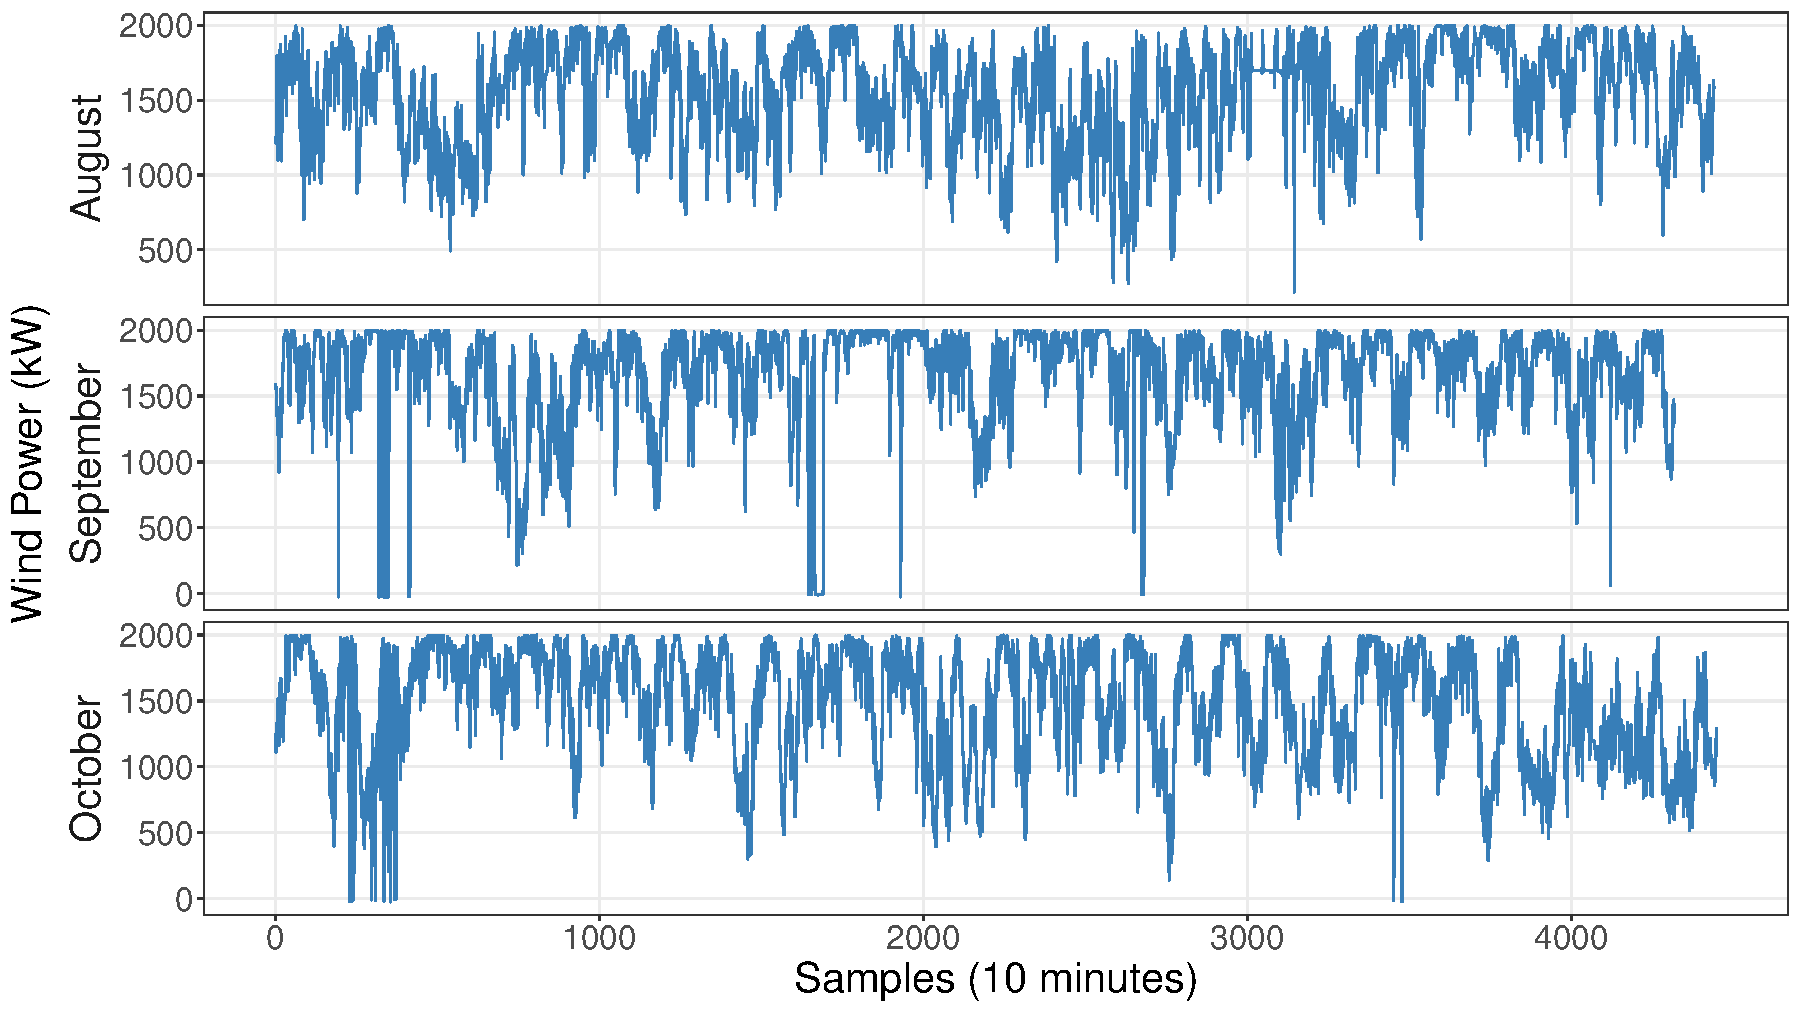
\includegraphics[width=\linewidth]{Media/cs2_datasets_plot.pdf}
    \caption{Datasets for August, September, and October 2017}
    \source{\citeonline{dasilva2021Novel}}
    \label{fig:datasetscs1}
\end{figure}

Further, the experiment split each dataset into training and test sets in the proportion of three weeks and one week, respectively. So, the test set (out-of-sample), comprising the last seven days of the month, have around 1,008 observations for each month. These proportions allow the models to learn the data pattern and behavior by using an adequate number of observations and make it possible to evaluate the learning in a sufficient number of values. Also, other proportions used in the literature were analysed such as 80 and 20\%, 75 and 25\%, and 70 and 30\%, however the proportion of three weeks for training set and one week for test was chosen due to interpretability and usability of the model by the company that provided the data. Table~\ref{tab:summary} presents an overview of the statistical indicators of the three datasets, which are mean, standard deviation (Std), minimum (Min), and maximum (Max).

\begin{landscape}
\begin{scriptsize}
\begin{center}
\begin{longtable}[htb!]{llllll|llll|llll}
\caption{Summary of the statistical indicators of the inputs and output of the datasets \label{tab:summary}} \\
\hline
\multirow{3}{*}{\textbf{Variable (Unit Measure)}} & \multirow{3}{*}{\textbf{Samples}} & \multicolumn{12}{c}{\textbf{Statistical indicator}} \\ \cline{3-14}
 & & \multicolumn{4}{c|}{August} & \multicolumn{4}{c|}{September} & \multicolumn{4}{c}{October} \\ \cline{3-14}
 & & Mean & Std & Min & Max & Mean & Std & Min & Max & Mean & Std & Min & Max \\ \hline \endfirsthead
  \multicolumn{14}{c}{\tablename\ \thetable\ -- \textit{Continued from previous page}} \\ \hline

\multirow{3}{*}{\textbf{Variable (Unit Measure)}} & \multirow{3}{*}{\textbf{Samples}} & \multicolumn{12}{c}{\textbf{Statistical indicator}} \\ \cline{3-14}
 & & \multicolumn{4}{c|}{August} & \multicolumn{4}{c|}{September} & \multicolumn{4}{c}{October} \\ \cline{3-14}
 & & Mean & Std & Min & Max & Mean & Std & Min & Max & Mean & Std & Min & Max \\ \hline \endhead \hline \multicolumn{14}{r}{\textit{Continued on next page}} \\
\endfoot
\hline
\endlastfoot

                                         
Power ($kW$)                             & Whole                    & 1553.02 & 338.82 & 217.5  & 2000.3 & 1652.78 & 395.46 & -24.7 & 2000.3 & 1478.57 & 422.85 & -25.3 & 2000.1 \\
                                         & Training                 & 1511.48 & 341.27 & 217.5  & 2000.3 & 1638.16 & 423.06 & -24.7 & 2000.3 & 1529.83 & 411.88 & -25.3 & 2000.1 \\
                                         & Test                     & 1694.46 & 288.64 & 572.4  & 2000.1 & 1700.81 & 281.57 & 61.4  & 2000.1 & 1303.64 & 413.11 & -24.8 & 1997.5 \\ \hline
Absolute Wind                            & Whole                    & 134.24  & 13.2   & 97.6   & 167.2  & 153.95  & 17.95  & 106.4 & 193.3  & 128.91  & 13.26  & 83.4  & 162.3  \\
Direction (Degrees)                      & Training                 & 134.31  & 13.28  & 97.6   & 167.2  & 159.46  & 15.81  & 106.4 & 193.3  & 130.36  & 12.01  & 93.9  & 160.9  \\
                                         & Test                     & 133.98  & 12.91  & 103.8  & 162.9  & 135.87  & 11.54  & 107.7 & 159.9  & 123.94  & 15.86  & 83.4  & 162.3  \\ \hline
Ambient Temperature                      & Whole                    & 26.04   & 2.49   & 22     & 32     & 25.75   & 2.61   & 22    & 32     & 26.51   & 2.63   & 23    & 33     \\
(Celsius)                                & Training                 & 25.94   & 2.44   & 22     & 31     & 25.66   & 2.57   & 22    & 32     & 26.37   & 2.66   & 23    & 33     \\
                                         & Test                     & 26.39   & 2.61   & 23     & 32     & 26.05   & 2.7    & 22    & 31     & 26.96   & 2.48   & 24    & 32     \\ \hline
Generator Bearing                        & Whole                    & 63.46   & 6.6    & 46     & 76     & 66.62   & 7.35   & 44    & 80     & 63.18   & 8.79   & 44    & 81     \\
Temperature (Celsius)                    & Training                 & 62.45   & 6.5    & 46     & 76     & 66.46   & 7.54   & 44    & 80     & 64.03   & 8.61   & 44    & 81     \\
                                         & Test                     & 66.89   & 5.69   & 50     & 75     & 67.17   & 6.65   & 50    & 78     & 60.27   & 8.77   & 46    & 79     \\ \hline
Generator Bearing 2                      & Whole                    & 49.98   & 4.59   & 39     & 59     & 51.44   & 4.9    & 39    & 60     & 50.03   & 5.64   & 38    & 64     \\
Temperature (Celsius)                    & Training                 & 49.38   & 4.55   & 39     & 59     & 51.3    & 4.96   & 39    & 60     & 50.55   & 5.6    & 38    & 64     \\
                                         & Test                     & 52.02   & 4.13   & 41     & 58     & 51.92   & 4.64   & 42    & 60     & 48.25   & 5.44   & 39    & 60     \\ \hline
Generator Speed (RPM)                    & Whole                    & 1282.16 & 75.08  & 335    & 1345.4 & 1293.32 & 169.49 & 0     & 1345.8 & 1253.17 & 121.96 & 0     & 1345.6 \\
                                         & Training                 & 1276.64 & 78.36  & 335    & 1345.4 & 1290.69 & 190.22 & 0     & 1345.8 & 1261.69 & 123.14 & 0     & 1345.6 \\
                                         & Test                     & 1300.94 & 58.87  & 1009.5 & 1345   & 1301.95 & 64.51  & 184.4 & 1345.1 & 1224.1  & 113.18 & 53.2  & 1344.9 \\ \hline
Nacelle Direction                        & Whole                    & 134.13  & 13.28  & 98.7   & 165.6  & 153.76  & 18.46  & 4.9   & 254.2  & 128.87  & 13.33  & 83.5  & 164    \\
(Degrees)                                & Training                 & 134.23  & 13.43  & 98.7   & 165.6  & 159.21  & 16.61  & 4.9   & 254.2  & 130.34  & 12.09  & 91.6  & 164    \\
                                         & Test                     & 133.78  & 12.74  & 104.2  & 161.9  & 135.87  & 11.69  & 109.4 & 162.1  & 123.88  & 15.91  & 83.5  & 160.4  \\ \hline
Wind Speed ($m/s$)                       & Whole                    & 9.24    & 1.18   & 5.1    & 15.4   & 10.5    & 1.67   & 5.2   & 17.2   & 9.02    & 1.32   & 4.7   & 13.8   \\
                                         & Training                 & 9.15    & 1.2    & 5.1    & 15.4   & 10.75   & 1.72   & 5.2   & 17.2   & 9.17    & 1.33   & 4.7   & 13.8   \\
                                         & Test                     & 9.52    & 1.06   & 6.3    & 12.6   & 9.69    & 1.14   & 6.5   & 13.3   & 8.52    & 1.14   & 5.4   & 12.5   \\ \hline
\end{longtable}
\end{center}
\end{scriptsize}
\end{landscape}

\subsection{Proposed Forecasting Framework}

The proposed model will be applied to train \ac{IMF}s and the residue generated by the decomposition step aiming to forecast the wind power generation in a multi-step-ahead forecasting strategy. Each dataset output was decomposed into five different \ac{IMF}s and one residue by \ac{CEEMD} (six components in total). The training process was performed by \ac{KNN}, \ac{PLS}, \ac{RIDGE}, and \ac{SVR} with the linear kernel as base-learners (weak model), and \ac{CUBIST} as meta-learner (strong model), for stack's layer-0 and layer-1, respectively, applied into each one of the six components. The component predictions in layer-0 are summed, giving four different predictions, one for each weak model. Those are applied as inputs for layer-1, where they were preprocessed using three other techniques: \ac{BC}, \ac{CORR}, and \ac{PCA}. The meta-learner training process of the three approaches was performed by \ac{CUBIST}, resulting in three proposed models, named \ac{CEEMD}--\ac{BC}--\ac{STACK}, \ac{CEEMD}--\ac{CORR}--\ac{STACK}, and \ac{CEEMD}--\ac{PCA}--\ac{STACK}, respectively. The step-by-step of the proposed methodology is given as follows:

\begin{enumerate}[start=1,label={\textbf{Step \arabic*:}},wide = 0pt, leftmargin = 3em]
\item The datasets' output variables are decomposed into five \ac{IMF}s and one residue by performing \ac{CEEMD} (six components). The datasets decomposition are illustrated in Figure~\ref{fig:IMFs}.

\begin{figure}[htb!]
    \centering
    \includegraphics[width=\linewidth]{Media/cs2_imf_plot}
    \caption{Datasets decomposed into IMFs and Residue by CEEMD}
    \source{\citeonline{dasilva2021Novel}}
    \label{fig:IMFs}
\end{figure}

\item The lag equals 4 was chosen, applied on the \ac{IMF}s creating four inputs from the lags, and lay on the exogenous inputs as well.

\item A \ac{BC} preprocess was applied on the \ac{IMF}s and the inputs in layer-0 of the stacking-ensemble learning.

\item Training each decomposition component with each base-learner model aforementioned using 5-fold cross-validation with a recurssive forecasting strategy.

\item A simple summation-grouping model reconstructed the component predictions. In other words, the components trained by the same base-learner model are summed \cite{dasilva2020Forecasting}. Then, four prediction outputs were generated named \ac{CEEMD}--\ac{KNN}, \ac{CEEMD}--\ac{PLS}, \ac{CEEMD}--\ac{RIDGE}, and \ac{CEEMD}--\ac{SVR}.

\item The four prediction outputs generated in layer-0 were used as input in layer-1. They were preprocessed using \ac{BC}, \ac{CORR} which removes those predictors whose correlation was greater than a threshold, and \ac{PCA}. Then, training each model using \ac{CUBIST} as meta-learner in layer-1 of the \ac{STACK} gives three different final predictions, which are the proposed models, named \ac{CEEMD}--\ac{BC}--\ac{STACK}, \ac{CEEMD}--\ac{CORR}--\ac{STACK}, and \ac{CEEMD}--\ac{PCA}--\ac{STACK}, respectively. To forecast 10, 20, and 30-minutes-ahead the applied structures are defined, respectively, as

\begin{scriptsize}
\begin{equation}
\hat{y}(t+h) = \begin{cases}
\hat{f}\left\{y(t+h-1),y(t+h-2),y(t+h-3),y(t+h-4),\mathbf{X}(t+h-1)\right\} & \text{if } h = 1, \\
\hat{f}\left\{\hat{y}(t+h-1),y(t+h-2),y(t+h-3),y(t+h-4),\mathbf{X}(t+h-2)\right\} & \text{if } h = 2, \\
\hat{f}\left\{\hat{y}(t+h-1),\hat{y}(t+h-2),y(t+h-3),y(t+h-4),\mathbf{X}(t+h-3)\right\} & \text{if } h = 3,
\end{cases}
\end{equation}
\end{scriptsize}
where $\hat{f}$ is a function that maps the wind power generation, $\hat{y}(t+h)$ is the forecast of wind power generation in horizon $h=$1 and 3 at time $t$ ($1,\ldots, 140$), $y(t+h-1)$, ${y}(t+h-2)$, ${y}(t+h-3)$, ${y}(t+h-4)$ are the previous observed, $\hat{y}(t+h-1)$, $\hat{y}(t+h-2)$ are the predicted wind power generation, $\mathbf{X}(t+h-n_x)$ is the exogenous inputs vector at the maximum lag of inputs ($n_x = 1$ if $h = 1$, {$n_x = 2$ if $h = 2$}, and $n_x = 3$ if $h = 3$).

\item Performance metrics (\ac{MAE}, \ac{MAPE}, and \ac{RMSE}) and statistical hypothesis tests (\ac{DM} test) were conducted to evaluate the accuracy of the proposed models compared to (i) different preprocess techniques applied in the layer-1 phase; (ii) \ac{CEEMD} models without \ac{STACK} method; (iii) \ac{STACK} models without decomposition and different preprocess techniques; and (iv) the models applied directly to the dataset. 

Hence, as described in this Section, the proposed model framework is illustrated in Figure~\ref{fig:frameworkcs1}.

% FIGURE - Framework
\begin{figure}[htb!]
    \centering
    \includegraphics[width=\textwidth]{Media/cs2_framework.pdf}
    \caption{Proposed forecasting framework for Application 2 \label{fig:frameworkcs1}}
    \source{\citeonline{dasilva2021Novel}}
\end{figure}

\end{enumerate}